%%% Ne pas modifier jusqu'à la ligne 25
\documentclass[a4paper,12pt]{book}
\usepackage[utf8]{inputenc}
\usepackage[french]{babel}
%%\usepackage{CJK}
\usepackage{yhmath}
\usepackage[left=2cm,right=2cm,top=3cm,bottom=2cm, headheight=1.5cm,headsep=1.5cm]{geometry}
%%\usepackage{CJKutf8}
\usepackage{amsfonts}
\usepackage{amsmath,amsfonts,amssymb,dsfont}
\usepackage{graphicx}
\usepackage{enumitem}		%\enumerate-resume
\usepackage[colorlinks=true,unicode={true},hyperindex=false, linkcolor=blue, urlcolor=blue]{hyperref}
\newcommand{\myref}[1]{\ref{#1} page \pageref{#1}}

\addto\captionsfrench{\def\tablename{Tableau}}  %légendes des tableaux
\renewcommand\thesection{\Roman{section}~-~} 
\renewcommand\thesubsection{\Roman{section}.\Alph{subsection}~-~} 
\renewcommand\thesubsubsection{\Roman{section}.\Alph{subsection}.\arabic{subsubsection}~-~} 

\newcommand{\conclusion}[1]{\newline \centerline{\fbox{#1}}}

\setcounter{secnumdepth}{3}
\parindent=0pt

\usepackage{fancyhdr}
\pagestyle{fancy}

\lhead{SJTU-ParisTech} 
%%%%%%%%%%%%%%%%%%%%%%%%%%%%%%%%%%
\chead{DM3}
\rhead{Daniel 518261910024}

\begin{document}
\renewcommand{\labelitemi}{$\blacktriangleright$}
\renewcommand{\labelitemii}{$\bullet$}


\section{Avancement et équilibre}
\begin{figure}[h]
    \begin{center}
    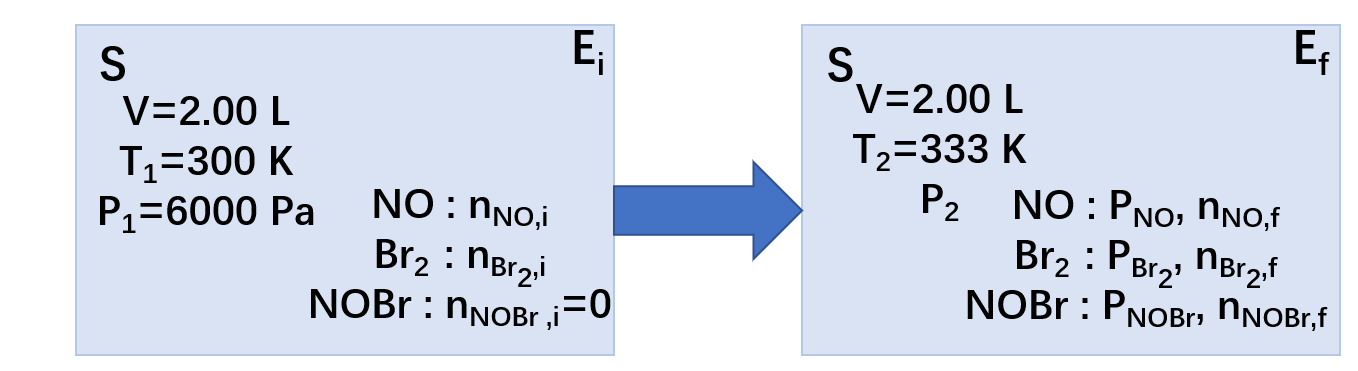
\includegraphics[scale=0.6]{dm3.png}
    \end{center}
    \caption{Figure du système étudié}
\end{figure}
\subsection{}
À l'état intial $E_i$, comme le $NO$ considéré comme gaz parfait idéal, on a 
$P_1V=n_{NO,i}RT_1$ car seulement le $NO$ est dans l'état gazeuse. 
On a donc $\boxed{n_{NO,i}=\frac{P_1V}{RT_1}}$. 

A.N. $\boxed{n_{NO,i}=\frac{6000*2.00*10^{-3}}{8.31*300}=4.81*10^{-3}\,mol}$

Et on a $\boxed{n_{Br_2,i}=\frac{m_{Br_2}}{M_{Br_2}}}$.
A.N. $\boxed{n_{Br_2,i}=\frac{300*10^{-6}}{159.8*10^{-3}}=1.88*10^{-3}\,mol}$
\subsection{}
Soit l’avancement de la réaction à l’équilibre $\xi_{eq}$. On note $n_{tot}$ le quantité de matière total à l’équilibre, 
et on a $P_2V=n_{tot}RT_2$ puisque tous les composants sont des gaz parfaits. 

\begin{table}[h]
\begin{center}
    \begin{tabular}{l|ccccc}
    \hline
                      & $2NO_{(g)}$      & + & $Br_{2(g)}$       & $\rightleftharpoons$ & $2NOBr_{(g)}$\\ \hline
        $n_{initial}$ & $n_{NO,i}$       &   & $n_{Br_2,i}$      &   & $n_{NOBr,i}=0$ \\ 
        $n_{eq}$      & $n_{NO,f}=n_{NO,i}-2\xi_{eq}$  &   & $n_{Br_2,f}=n_{Br_2,i}-\xi_{eq}$  &   & $n_{NOBr,f}=2\xi_{eq}$ \\ 
    \end{tabular}
\end{center}
\end{table}

À l’équilibre, on a $K^\circ(T_2)=Q_{eq}$, donc 

\begin{align*}
    K^\circ(T_2)       &=\frac{a(NOBr)^2}{a(NO)^2a(Br_2)}\\
                       &=\frac{\left(\frac{P_{NOBr}}{P^\circ}\right)^2}{\left(\frac{P_{NO}}{P^\circ}\right)^2\left(\frac{P_{Br_2}}{P^\circ}\right)}\\
                       &=\frac{\left(\frac{n_{NOBr}}{n_{tot}}P_2\right)^2P^\circ}{\left(\frac{n_{NO}}{n_{tot}}P_2\right)^2\left(\frac{n_{Br_2}}{n_{tot}}P_2\right)}\\
                       &=\frac{P^\circ V n^2_{NOBr_2,f}}{RTn^2_{NO,f}n_{Br_2,f}}\\
                       &=\frac{P^\circ V (2\xi_{eq})^2}{RT(n_1-2\xi_{eq})^2(n_2-\xi_{eq})}
\end{align*}
On a $K^\circ(T_2)=13.2$, et il faut $\xi_{eq}<\xi_{max}=n_{Br_2,i}$. A.N. On a $\boxed{\xi_{eq}=7.51*10^{-4}\,mol}$
\subsection{}
On a $n_{tot}=n_{NO,f}+n_{Br_2,f}+n_{NOBr,f}=n_{NO,i}+n_{Br_2,i}-\xi_{eq}$. 
Par l'équation du gaz parfait, $\boxed{P_2=\frac{n_{tot}RT_2}{V}=\frac{(n_{NO,i}+n_{Br_2,i}-\xi_{eq})RT_2}{V}}$

A.N. $\boxed{P_2=\frac{(4.81*10^{-3}+1.88*10^{-3}-7.51*10^{-4})*8.31*333}{2.00*10^{-3}}=8.22*10^{3}\,Pa}$

\end{document}